\documentclass{beamer}
\usepackage{verbatim}
\usepackage{xcolor}
\usepackage{multirow}
%\usepackage{enumitem}
\usetheme{Warsaw}
\setbeamertemplate{navigation symbols}{}
\newcommand{\blue}[1]{{\color{blue} #1}}
\newcommand{\red}[1]{{\color{red} #1}}
\newcommand{\bluRed}[2]{{\color{blue} #1}{\color{red} #2}}
\newcommand{\qtns}[0]{\begin{center} Questions? \end{center}}
\newcommand{\nl}[1]{\vspace{#1 em}}
\newcommand{\cntrImg}[2]{\begin{center}\includegraphics[scale=#2]{#1}\end{center}}

\title{Math 3070, Applied Statistics}

\begin{document}

\begin{frame}
    \begin{beamercolorbox}[rounded=true,wd=\textwidth,center]{title}
        \usebeamerfont{title}\inserttitle
    \end{beamercolorbox}
    \begin{center}
        Section 1\\
        \nl{0.5}
        August 19, 2019
    \end{center}

\end{frame}

\begin{frame}{Syllabus}
    \begin{itemize}
        \item Course structure
        \item Office hours
        \item Materials and canvas
        \item Lab requirement, {\bf you need to pass both for credit}
        \item Grading, homework, quizzes, exams
        \item Calendar
    \end{itemize}
\end{frame}

\begin{frame}{Lecture Style}
    \begin{itemize}
        \item Defintion(s)/Method/Explanation(s) $\rightarrow$ example(s) $\rightarrow$ comments and questions
        \item {\bf Definitions} are in bold.
        \item {\it Math jargon} is italicized. You don't need to know these terms in this , but they frequently show up in other math work.
        \item \blue{Color} \red{coding} will be used to highlight different ingredients of a method. Will be dropped after the first one or two examples.
        \item Sections from the book will be written in the title of the first relevant slide.
    \end{itemize}
\end{frame}

\begin{frame}{Lecture Outline, 8/12}
    \begin{itemize}
        \item 1.1 Statistical nomenclature
        \item 1.1 Sampling methods
        \item 1.2 Pictorial and tabular methods in descriptive statistics
    \end{itemize}
\end{frame}

\begin{frame}{Statistical nomenclature, Section 1.1}
    \begin{itemize}
        \item {\bf Population}: group of interest.
        \item {\bf Data}: collection of facts, usually about the population.
        \item {\bf Quantitative data}: data which are numbers. Example: length, weight, volume and etc.
        \item {\bf Quantitative data}: data which are categories. Example: open or close; color; dead, alive, dead, or undead; and etc.
        \item {\bf Census}: Data of the entire population
        \item {\bf Sample}: Data of a subset of the population. Most data is sample data. Sampling means to generate a sample.
        \item Sample data is compromised of observations consisting of variables, quantities/characteristics of interest.
        \item {\bf Univariate} (data): Observations measure one variable
        \item {\bf Multivariate} (data): Observations measure more than one variable(s)
        \item {\bf Bivariate} (data): Observations measure exactly two variables
    \end{itemize}
\end{frame}

\begin{frame}{Statistical nomenclature}
    \begin{itemize}
        \item {\bf Enumerative Studies}: Studies of an existing fixed, finite population. Example, meauring plant heights or coin flips.
        \item {\bf Analytic Studies}: Studies of a process which may not exist. Example, developing methods for measuring variance of plant heights or coin flips.
    \end{itemize}
\end{frame}

\begin{frame}{Sampling Methods}
    \begin{itemize}
        \item {\bf Bias} (statistical): Source of incorrect measurement of population characteristics. Example, sampling only NBA players to determine the average height of a US citizen.
        \item {\bf Simple Random Sampling }(SRS): samlping method were each member of the population of interest is eligible to be randomly selected to be included in the sample.
        \item {\bf Strata}: Partitions of a population based on similar traits. Example, grouping dogs based on fur color; hair color is the strata.
        \item {\bf Stratified Sampling}: sampling method were the population is divided into observable strata. Used to avoid under-representation.
        \item {\bf Convenience Sampling}: Sampling which to prioritizes convenience, usually not random and has bias. Example, poll only our classmates when the population of interest is all students at the U.
    \end{itemize}
\end{frame}

\begin{frame}{Recurring Definitions}
    \begin{itemize}
        \item Quantitative data can be categorized into discrete and continuous data.
        \item {\bf discrete}: Number of observable or possible values of data are countable or finite. Example, number of days in a month, number of times a coin lands on heads in 50 flips, heights of students rounded to the nearest inch, any integer and etc.
        \item {\bf continuous}: Observable or possible values consist of entire intervals. Example, heights unrounded, weights of shipping containers, any number between 0 and 1 and etc. On a computer all data is discrete, but if each number appears once, the data should be treated as continuous.
    \end{itemize}
\end{frame}

\begin{frame}{Recurring Definitions}
    \begin{itemize}
        \item {\bf Sample Size}: number of observations in a sample.
        \item Population, sample, sample size, data, categorical and quantitative variables (discrete and continuous), observations will appear throughout.
        \item {\bf Probability}: The field of mathematics that describes the behavior of objects in the presence (or lack of) uncertainty or randomness.
        \item {\bf Distribution}:  What values a variable takes and how frequently it takes them. Can express the distribution of  data in plots or model the dsitribution of probabilistic objects as a {\it generalized} function, called a distribution.
    \end{itemize}
\end{frame}

\begin{frame}{Pictorial and Tabular Methods in Descriptive Statistics, Section 1.2}
    Given quantitative data (should be discrete), the distribution can be described using the following:
    \begin{itemize}
        \item Stem-and-Leaf Plot
        \item Dot Plot
        \item Frequency Distribution
        \item Histogram
    \end{itemize}
\end{frame}

\begin{frame}{Stem-and-Leaf Plot, Method}
    Construction
    \begin{enumerate}
        \item Select the \blue{leading} digits to be \blue{stem} digits and \red{remianing} digits to be \red{leaf} digits.
        \item Draw a vertical line with the \blue{stem} digits on the left.
        \item Record the corresponding \red{leaf} values to right of the line.
        \item Indicate the units of the \red{stem} and \blue{leaf} digits.
    \end{enumerate}
\end{frame}

\begin{frame}{Stem-and-Leaf Plot, Example}
    Data: number of heads in 100 coin flips. Discrete, quantitative data
    \[63,47,52,54,50,
        57,39,41,49,49,
        50, 52, 55, 51, 56,
        53, 47, 49, 50, 62 \]
    \begin{center}
        Sample size $= 20$
    \end{center}
\end{frame}

\begin{frame}{Stem-and-Leaf Plot, Example}
    Step 1: Select the \blue{leading} digits to be \blue{stem} digits and \red{remianing} digits to be \red{leaf} digits.
    \[\bluRed{6}{3},
        \bluRed{4}{7},
        \bluRed{5}{2},
        \bluRed{5}{4},
        \bluRed{5}{0},
        \bluRed{5}{7},
        \bluRed{3}{9},
        \bluRed{4}{1},
        \bluRed{4}{9},
        \bluRed{4}{9},
        \bluRed{5}{0},
        \bluRed{5}{2},
        \bluRed{5}{5},
        \bluRed{5}{1},
        \bluRed{5}{6},
        \bluRed{5}{3},
        \bluRed{5}{4},
        \bluRed{4}{9},
        \bluRed{5}{0},
        \bluRed{6}{2}, \]
\end{frame}

\begin{frame}{Stem-and-Leaf Plot, Example}
    Step 2: Draw a vertical line with the \blue{stem} digits on the left.
    \[\bluRed{6}{3},
        \bluRed{4}{7},
        \bluRed{5}{2},
        \bluRed{5}{4},
        \bluRed{5}{0},
        \bluRed{5}{7},
        \bluRed{3}{9},
        \bluRed{4}{1},
        \bluRed{4}{9},
        \bluRed{4}{9},
        \bluRed{5}{0},
        \bluRed{5}{2},
        \bluRed{5}{5},
        \bluRed{5}{1},
        \bluRed{5}{6},
        \bluRed{5}{3},
        \bluRed{5}{4},
        \bluRed{4}{9},
        \bluRed{5}{0},
        \bluRed{6}{2}\]
    \begin{table}
        \begin{tabular}{r | l}
            \blue{6} & \\
            \blue{5} & \\
            \blue{4} & \\
            \blue{3} & \\
        \end{tabular}
    \end{table}
\end{frame}


\begin{frame}{Stem-and-Leaf Plot, Example}
    Step 3: Record the corresponding \red{leaf} values to right of the line.
    \[\bluRed{6}{3},
        \bluRed{4}{7},
        \bluRed{5}{2},
        \bluRed{5}{4},
        \bluRed{5}{0},
        \bluRed{5}{7},
        \bluRed{3}{9},
        \bluRed{4}{1},
        \bluRed{4}{9},
        \bluRed{4}{9},
        \bluRed{5}{0},
        \bluRed{5}{2},
        \bluRed{5}{5},
        \bluRed{5}{1},
        \bluRed{5}{6},
        \bluRed{5}{3},
        \bluRed{5}{4},
        \bluRed{4}{9},
        \bluRed{5}{0},
        \bluRed{6}{2}\]
    \begin{table}
        \begin{tabular}{r | l}
            \blue{6} & \red{23}           \\
            \blue{5} & \red{000122344567} \\
            \blue{4} & \red{17999}        \\
            \blue{3} & \red{9}            \\
        \end{tabular}
    \end{table}
\end{frame}

\begin{frame}{Stem-and-Leaf Plot, Example}
    Step 4: Indicate the units of the \red{stem} and \blue{leaf} digits.
    \[\bluRed{6}{3},
        \bluRed{4}{7},
        \bluRed{5}{2},
        \bluRed{5}{4},
        \bluRed{5}{0},
        \bluRed{5}{7},
        \bluRed{3}{9},
        \bluRed{4}{1},
        \bluRed{4}{9},
        \bluRed{4}{9},
        \bluRed{5}{0},
        \bluRed{5}{2},
        \bluRed{5}{5},
        \bluRed{5}{1},
        \bluRed{5}{6},
        \bluRed{5}{3},
        \bluRed{5}{4},
        \bluRed{4}{9},
        \bluRed{5}{0},
        \bluRed{6}{2}\]
    \begin{table}
        \begin{tabular}{r | l}
            \blue{6} & \red{23}           \\
            \blue{5} & \red{000122344567} \\
            \blue{4} & \red{17999}        \\
            \blue{3} & \red{9}            \\
        \end{tabular}
    \end{table}
    \blue{stem units: tens}\\
    \red{leaf units: ones}
\end{frame}

\begin{frame}{Stem-and-Leaf Plot, Example}
    Step 4: Indicate the units of the \red{stem} and \blue{leaf} digits.
    \[\bluRed{6}{3},
        \bluRed{4}{7},
        \bluRed{5}{2},
        \bluRed{5}{4},
        \bluRed{5}{0},
        \bluRed{5}{7},
        \bluRed{3}{9},
        \bluRed{4}{1},
        \bluRed{4}{9},
        \bluRed{4}{9},
        \bluRed{5}{0},
        \bluRed{5}{2},
        \bluRed{5}{5},
        \bluRed{5}{1},
        \bluRed{5}{6},
        \bluRed{5}{3},
        \bluRed{5}{4},
        \bluRed{4}{9},
        \bluRed{5}{0},
        \bluRed{6}{2}\]
    \begin{table}
        \begin{tabular}{r | l}
            \blue{6} & \red{23}           \\
            \blue{5} & \red{000122344567} \\
            \blue{4} & \red{17999}        \\
            \blue{3} & \red{9}            \\
        \end{tabular}
    \end{table}
    \blue{stem units: tens}\\
    \red{leaf units: ones}
\end{frame}

\begin{frame}{Stem-and-Leaf Plot, Second Example}
    Data: proportion of water in different drinks, rounded to nearest hundredths.
    \[\bluRed{0.7}{3},
        \bluRed{0.7}{9},
        \bluRed{0.6}{1},
        \bluRed{0.0}{6},
        \bluRed{0.4}{1},
        \bluRed{0.2}{6},
        \bluRed{0.9}{0},
        \bluRed{0.0}{7},
        \bluRed{0.5}{2},
        \bluRed{0.9}{3},
        \bluRed{0.3}{9},
        \bluRed{0.7}{2}\]
    \begin{table}
        \begin{tabular}{r | l}
            \blue{0.9} & \red{0 3}   \\
            \blue{0.8} & \red{}      \\
            \blue{0.7} & \red{2 3 9} \\
            \blue{0.6} & \red{1}     \\
            \blue{0.5} & \red{2}     \\
            \blue{0.4} & \red{1}     \\
            \blue{0.3} & \red{9}     \\
            \blue{0.2} & \red{6}     \\
            \blue{0.1} & \red{}      \\
            \blue{0.0} & \red{6 7}   \\
        \end{tabular}
    \end{table}
    \blue{stem units: tenths}\\
    \red{leaf units: hundredths}
\end{frame}

\begin{frame}{Stem-and-Leaf Plot, Comments/Questions}
    \begin{itemize}
        \item Shows visual shape of of the distribution (of data).
        \item Displays observed values
        \item Usually better for discrete data. Truly continuous will usually display one observation at each value.
    \end{itemize}
    \qtns
\end{frame}

\begin{frame}{Stem-and-Leaf Plot, Comments and Questions}
    \begin{itemize}
        \item Shows visual shape of of the distribution
        \item Displays observed values
        \item Usually better for discrete data. Truly continuous will usually display one observation at each value.
    \end{itemize}
    \qtns
\end{frame}

\begin{frame}{Stem-and-Leaf Plot, Comments/Questions}
    \begin{itemize}
        \item Shows visual shape of of the distribution
        \item Displays observed values
        \item Usually better for discrete data. Truly continuous will usually display one observation at each value.
    \end{itemize}
    \qtns
\end{frame}

\begin{frame}{Dot Plot, Explanation and Example}
    Dot plots are simliar to stem-and-leaf plots, except they have a hortizonal bar and there are dots instead of leaf digits.\\
    \nl{0.5}
    Example Data: Concrete flexural strength (in MPa) rounded to nearest tenth. Discrete quantitative data.
    \[5.9,6.3,6.3,6.5,6.8,6.8,7.0,7.0,7.2,7.3,7.4,7.6,7.7,7.7,\]
    \[7.8,7.8,7.9,8.1,8.2,8.7,9.0,9.7,9.7,10.7,11.3,11.6,11.8\]
    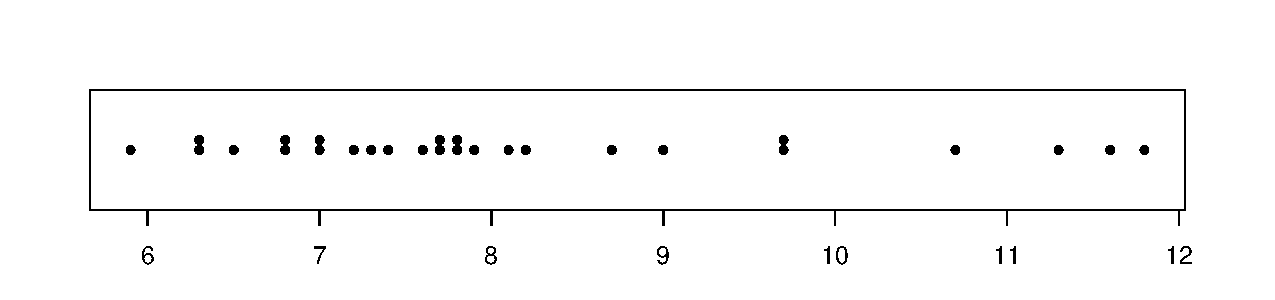
\includegraphics[scale=.5]{ch01_strength_dot_stack.pdf}
\end{frame}

\begin{frame}{Dot Plot, Comments and Questions}
    \begin{itemize}
        \item Only shows the visual shape of the distribution (of data), values not quickly readable.
        \item Should be used with discrete data.
        \item Less informative than stem-and-leaf plots, but more visually pleasing.
    \end{itemize}
    \qtns
\end{frame}

\begin{frame}{Frequency Distribution, Definitions}
    \begin{itemize}
        \item {\bf Frequency}: Number of times a value is observed in a data set. Should be used with discrete data; continuous data usually reports each number once.
        \item {\bf Relative Frequency}: Frequency of a value divide by the sample size.
        \item {\bf Frequency Distribution}: Table of frequencies or relative frequencies at each observed value.
    \end{itemize}
\end{frame}

\begin{center}
    \begin{frame}{Frequency Distribution, Example}
        Data: Value of a dice roll, 20 rolls. Quantitative, discrete data.
        \[4,4,3,3,2,4,6,3,6,6\]
        \[1,2,6,3,1,3,5,5,2,2\]
        \blue{frequency of $4$ = 3} \hskip 1em
        \red{sample size = 20}
        \[\mbox{relative frequency of }4 = \frac{\blue{\mbox{frequency of }4}}{\mbox{\red{sample size}}} = \frac{\blue{3}}{\red{20}}=0.15\]
        \begin{tabular}{|l | r | r| r | r | r | r|}
            \hline
            dice roll          & 1        & 2        & 3        & 4        & 5        & 6         \\
            \hline
            \blue{frequency}   & \blue{2} & \blue{4} & \blue{5} & \blue{3} & \blue{2} & \blue{4 } \\
            \hline
            relative frequency & 0.10     & 0.20     & 0.25     & 0.15     & 0.10     & 0.20      \\
            \hline
        \end{tabular}
    \end{frame}
\end{center}

\begin{center}
    \begin{frame}{Frequency Distribution, Comments and Questions}
        \begin{center}
            Works well with discrete data.
        \end{center}
        \qtns
    \end{frame}
\end{center}

\begin{frame}{Histogram, Method}
    \begin{center}
        Histograms are appropriately visually quantitative, continuous data. Moreover, they can be used with discrete data as well.
    \end{center}
    {\bf bins}: Intervals, usually equal length and consecutive. Most commonly, the left endpoint is excluded and the right endpoint is included.
    \begin{enumerate}
        \item On a a segment of the number line, draw bins so that your each datum lies within a bins.
        \item Within each bin draw a bar extending to the number of data observed in the bin, or the frequency of obervations in the bin.
    \end{enumerate}
\end{frame}

\begin{frame}{Histogram, Example}
    Data: Energy consumption of homes (BTU). Quantitative, continuous data. (Technically, the data is rounded, but each number only appears roughly once so it can be thought of as continuous.)\\
    \nl{0.5}
    2.97,
    4.00,
    5.20,
    5.56,
    5.94,
    5.98,
    6.35,
    6.62,
    6.72,
    6.78,
    6.80,
    6.85,
    6.94,
    7.15,
    7.16,
    7.23,
    7.39,
    7.62,
    7.62,
    7.69,
    7.73,
    7.87,
    7.93,
    8.00,
    8.26,
    8.29,
    8.37,
    8.47,
    8.56,
    8.58,
    8.61,
    8.67,
    8.69,
    8.81,
    9.07,
    9.27,
    9.37,
    9.43,
    9.52,
    9.58,
    9.60,
    9.76,
    9.82,
    9.83,
    9.83,
    9.84,
    9.96,
    10.04,
    10.21,
    10.28,
    10.28,
    10.30,
    10.35,
    10.36,
    10.40,
    10.49,
    10.50,
    10.64,
    10.95,
    11.09,
    11.12,
    11.21,
    11.29,
    11.43,
    11.62,
    11.70,
    11.70,
    12.16,
    12.19,
    12.28,
    12.31,
    12.62,
    12.69,
    12.71,
    12.91,
    12.92,
    13.11,
    13.38,
    13.42,
    13.43,
    13.47,
    13.60,
    13.96,
    14.24,
    14.35,
    15.12,
    15.24,
    16.06,
    16.90,
    18.26
\end{frame}

\begin{frame}{Histogram, Example}
    Step 1: On a a segment of the number line, draw bins so that your each datum lies within a bin. \\
    \nl{0.5}
    The following interval contain all following bins:\\ \nl{0.5}
    $(0,2]$,
    $(2,4]$,
    $(4,6]$,
    $(6,8]$,
    $(8,10]$,
    $(10,12]$,
    $(12,14]$,
    $(14,16]$,
    $(16,18]$,
    $(18,20]$
\end{frame}

\begin{frame}{Histogram, Example}
    Step 2: Within each bin draw a bar extending to the number of data observed in the bin, or the frequency of obervations in the bin.
    \cntrImg{ch01_power_hist.pdf}{0.4}
\end{frame}

\begin{frame}{Histogram, Comments and Questions}
    \begin{itemize}
        \item Can be used with continuous and discrete quantitative data.
        \item Shows shape of distribution.
    \end{itemize}
    What if we used a dot plot?
    \cntrImg{ch01_power_dot_stack.pdf}{0.5}
    Hard to see the shape of the data, no bins.
    \qtns
\end{frame}

\begin{frame}{Visualizing Categorical Data}
    \begin{itemize}
        \item bar plots, bars show frequency of observations
        \item frequency or relative frequency tables
    \end{itemize}
\end{frame}

\end{document}